
\newpage
\appendix
\thispagestyle{plain}
\section{VCA vs. VCA Competition}
We include the following figures to demonstrate that most VCAs can achieve their
nominal uplink utilization rate when in competition with the other VCAs on a 
3 Mbps uplink capacity, the minimum uplink capacity recommended by the FCC (25/3). 
The only exception is two competing Teams calls, which we discuss in Section 5. 
\FloatBarrier

\setcounter{figure}{0}
\renewcommand\thefigure{A.\arabic{figure}}

\setcounter{table}{0}
\renewcommand\thetable{A.\arabic{table}}

\begin{figure}[]
\centering
\begin{subfigure}[t]{.4\textwidth}
    \centering
    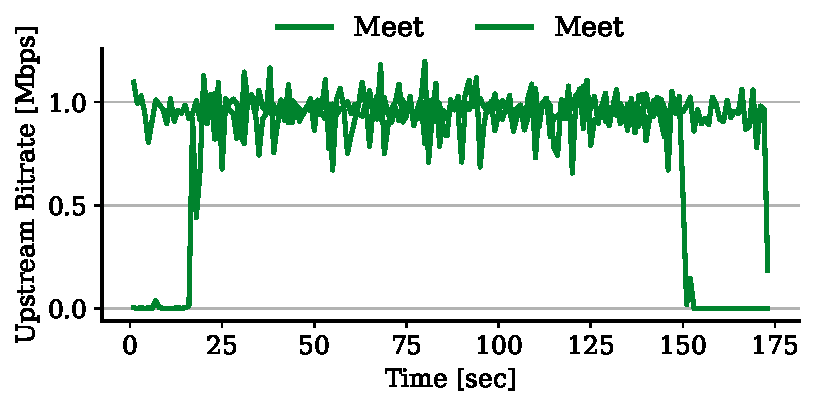
\includegraphics[width=1\textwidth]{figures/appendix/meet_meet_3_ul_r2.pdf}
    \caption{Meet vs. Meet}
    \label{subfig:meet-meet-3}
\end{subfigure}\hfill
\begin{subfigure}[t]{.4\textwidth}
    \centering
    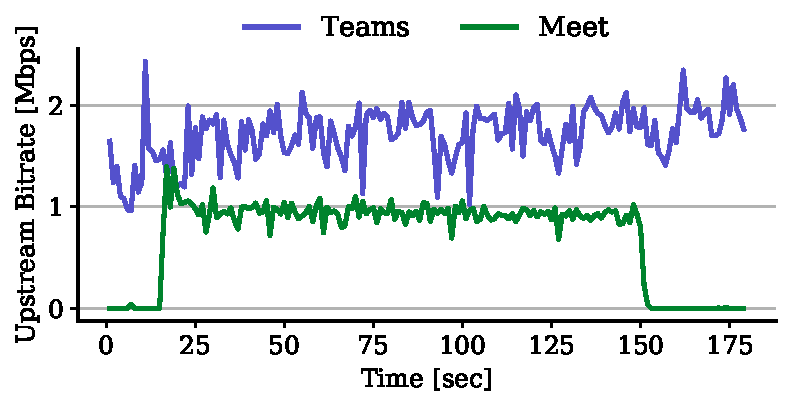
\includegraphics[width=1\textwidth]{figures/appendix/teams_meet_3_ul_r3.pdf}
    \caption{Teams vs. Meet}
    \label{subfig:teams-meet-3}
\end{subfigure}
\begin{subfigure}[t]{.4\textwidth}
    \centering
    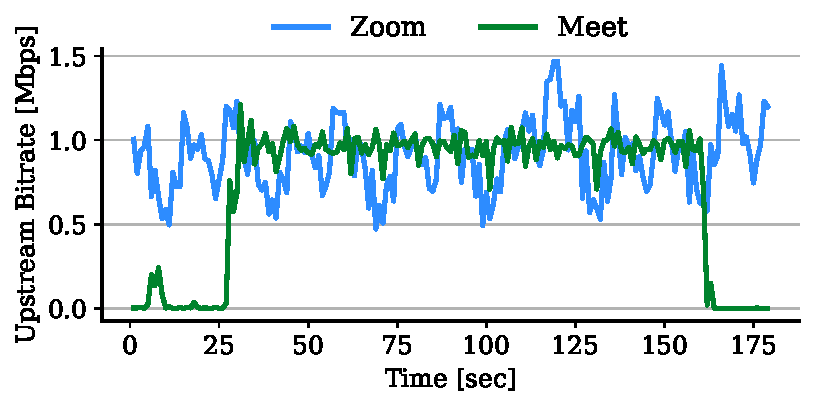
\includegraphics[width=1\textwidth]{figures/appendix/zoom_meet_3_ul_r2.pdf}
    \caption{Zoom vs. Meet}
    \label{subfig:zoom-meet-3}
\end{subfigure}
\begin{subfigure}[t]{.4\textwidth}
    \centering
    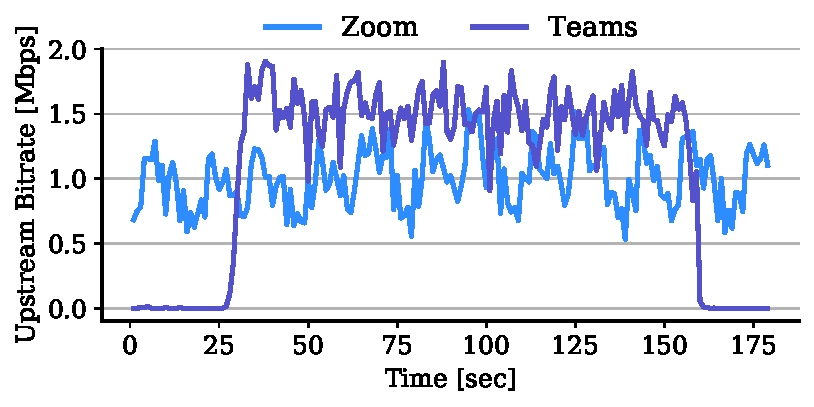
\includegraphics[width=1\textwidth]{figures/appendix/zoom_teams_3_ul_r2.pdf}
    \caption{Zoom vs. Teams}
    \label{subfig:zoom-teams-3}
\end{subfigure}
\begin{subfigure}[t]{.4\textwidth}
    \centering
    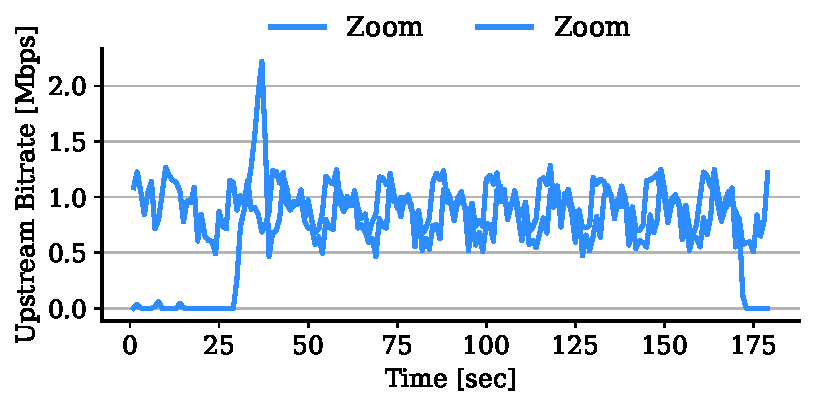
\includegraphics[width=1\textwidth]{figures/appendix/zoom_zoom_3_ul_r1.pdf}
    \caption{Zoom vs. Zoom}
    \label{subfig:zoom-zoom-3}
\end{subfigure}
\caption{VCA vs. VCA on a 3 Mbps symmetric connection.}
\label{fig:vca-vca-3}
\end{figure}